\documentclass[a4paper,14pt]{article}\usepackage[]{graphicx}\usepackage[]{color}
%% maxwidth is the original width if it is less than linewidth
%% otherwise use linewidth (to make sure the graphics do not exceed the margin)
\makeatletter
\def\maxwidth{ %
  \ifdim\Gin@nat@width>\linewidth
    \linewidth
  \else
    \Gin@nat@width
  \fi
}
\makeatother

\definecolor{fgcolor}{rgb}{0.345, 0.345, 0.345}
\newcommand{\hlnum}[1]{\textcolor[rgb]{0.686,0.059,0.569}{#1}}%
\newcommand{\hlstr}[1]{\textcolor[rgb]{0.192,0.494,0.8}{#1}}%
\newcommand{\hlcom}[1]{\textcolor[rgb]{0.678,0.584,0.686}{\textit{#1}}}%
\newcommand{\hlopt}[1]{\textcolor[rgb]{0,0,0}{#1}}%
\newcommand{\hlstd}[1]{\textcolor[rgb]{0.345,0.345,0.345}{#1}}%
\newcommand{\hlkwa}[1]{\textcolor[rgb]{0.161,0.373,0.58}{\textbf{#1}}}%
\newcommand{\hlkwb}[1]{\textcolor[rgb]{0.69,0.353,0.396}{#1}}%
\newcommand{\hlkwc}[1]{\textcolor[rgb]{0.333,0.667,0.333}{#1}}%
\newcommand{\hlkwd}[1]{\textcolor[rgb]{0.737,0.353,0.396}{\textbf{#1}}}%
\let\hlipl\hlkwb

\usepackage{framed}
\makeatletter
\newenvironment{kframe}{%
 \def\at@end@of@kframe{}%
 \ifinner\ifhmode%
  \def\at@end@of@kframe{\end{minipage}}%
  \begin{minipage}{\columnwidth}%
 \fi\fi%
 \def\FrameCommand##1{\hskip\@totalleftmargin \hskip-\fboxsep
 \colorbox{shadecolor}{##1}\hskip-\fboxsep
     % There is no \\@totalrightmargin, so:
     \hskip-\linewidth \hskip-\@totalleftmargin \hskip\columnwidth}%
 \MakeFramed {\advance\hsize-\width
   \@totalleftmargin\z@ \linewidth\hsize
   \@setminipage}}%
 {\par\unskip\endMakeFramed%
 \at@end@of@kframe}
\makeatother

\definecolor{shadecolor}{rgb}{.97, .97, .97}
\definecolor{messagecolor}{rgb}{0, 0, 0}
\definecolor{warningcolor}{rgb}{1, 0, 1}
\definecolor{errorcolor}{rgb}{1, 0, 0}
\newenvironment{knitrout}{}{} % an empty environment to be redefined in TeX

\usepackage{alltt}
\usepackage[paperwidth=21cm,paperheight=29.7cm,top=3cm,right=1.5cm,bottom=3cm,left=1.5cm]{geometry}
\usepackage{makeidx}
%\usepackage{CJKutf8}
%\usepackage{xeCJK}
%\usepackage{multirow}
%\usepackage{multicol}
%\usepackage[dvipsnames,svgnames,table]{xcolor}
\usepackage{graphicx}
\usepackage{epstopdf}
\usepackage{ulem}
\usepackage{amsmath}
\usepackage{amssymb}
\usepackage{fontspec}
\usepackage[toc,page]{appendix}
\usepackage{pdflscape}
\usepackage{supertabular}
\usepackage{dcolumn}
%\setCJKmainfont{標楷體}
\author{Oscar Deng}
\title{企業競爭策略與產業競爭程度對避稅行為之影響}
\date{\today}
\IfFileExists{upquote.sty}{\usepackage{upquote}}{}
\begin{document}
%\begin{CJK}{UTF8}{kaiu}
\tableofcontents
\maketitle
\appendix
\section{\\Appendix A: Preparing everything} \label{App:Appendix A}
\begin{knitrout}
\definecolor{shadecolor}{rgb}{0.969, 0.969, 0.969}\color{fgcolor}\begin{kframe}
\begin{alltt}
\hlcom{#source("setSweave.R")}
\hlcom{#source("setSweave.big5.R")}
\hlkwd{require}\hlstd{(stargazer)}
\end{alltt}


{\ttfamily\noindent\itshape\color{messagecolor}{\#\# Loading required package: stargazer}}

{\ttfamily\noindent\itshape\color{messagecolor}{\#\# \\\#\# Please cite as:}}

{\ttfamily\noindent\itshape\color{messagecolor}{\#\#\ \ Hlavac, Marek (2015). stargazer: Well-Formatted Regression and Summary Statistics Tables.}}

{\ttfamily\noindent\itshape\color{messagecolor}{\#\#\ \ R package version 5.2. http://CRAN.R-project.org/package=stargazer}}\begin{alltt}
\hlkwd{require}\hlstd{(xtable)}
\end{alltt}


{\ttfamily\noindent\itshape\color{messagecolor}{\#\# Loading required package: xtable}}\begin{alltt}
\hlkwd{require}\hlstd{(dplyr)}
\end{alltt}


{\ttfamily\noindent\itshape\color{messagecolor}{\#\# Loading required package: dplyr}}

{\ttfamily\noindent\itshape\color{messagecolor}{\#\# \\\#\# Attaching package: 'dplyr'}}

{\ttfamily\noindent\itshape\color{messagecolor}{\#\# The following objects are masked from 'package:stats':\\\#\# \\\#\#\ \ \ \  filter, lag}}

{\ttfamily\noindent\itshape\color{messagecolor}{\#\# The following objects are masked from 'package:base':\\\#\# \\\#\#\ \ \ \  intersect, setdiff, setequal, union}}\begin{alltt}
\hlkwd{require}\hlstd{(data.table)}
\end{alltt}


{\ttfamily\noindent\itshape\color{messagecolor}{\#\# Loading required package: data.table}}

{\ttfamily\noindent\itshape\color{messagecolor}{\#\# -------------------------------------------------------------------------}}

{\ttfamily\noindent\itshape\color{messagecolor}{\#\# data.table + dplyr code now lives in dtplyr.\\\#\# Please library(dtplyr)!}}

{\ttfamily\noindent\itshape\color{messagecolor}{\#\# -------------------------------------------------------------------------}}

{\ttfamily\noindent\itshape\color{messagecolor}{\#\# \\\#\# Attaching package: 'data.table'}}

{\ttfamily\noindent\itshape\color{messagecolor}{\#\# The following objects are masked from 'package:dplyr':\\\#\# \\\#\#\ \ \ \  between, last}}\begin{alltt}
\hlkwd{require}\hlstd{(ggplot2)}
\end{alltt}


{\ttfamily\noindent\itshape\color{messagecolor}{\#\# Loading required package: ggplot2}}\begin{alltt}
\hlkwd{require}\hlstd{(stats)}
\hlkwd{source}\hlstd{(}\hlstr{"corstars.R"}\hlstd{)}
\hlstd{TEJ8.1} \hlkwb{<-} \hlkwd{read.csv}\hlstd{(}\hlstr{"TEJ8.1.csv"}\hlstd{,}\hlkwc{row.names} \hlstd{=} \hlnum{1}\hlstd{)}
\end{alltt}
\end{kframe}
\end{knitrout}

\newpage
\section{\\Appendix D.1: Descriptive Statistics Table} \label{App:Appendix D.1}
\begin{kframe}
\begin{alltt}
\hlkwd{stargazer}\hlstd{(}
    \hlstd{TEJ8.1} \hlopt \hlkwd{select}\hlstd{(ETR,CETR,STR,HHI_Dum,STR_HHI,ROA,SIZE,LEV,}
                      \hlstd{INTANG,QUICK,EQINC,OUTINSTI,RELAT,FAM_Dum,GDP,}
                      \hlcom{#,RD,EMP,MB,MARKET,PPE}
                      \hlstd{STR_RD,STR_EMP,STR_MB,STR_MARKET,STR_PPE}
                      \hlstd{)}
 \hlstd{,}\hlkwc{type} \hlstd{=} \hlstr{"latex"}
 \hlstd{,}\hlkwc{summary.stat} \hlstd{=} \hlkwd{c}\hlstd{(}\hlstr{"n"}\hlstd{,}\hlstr{"min"}\hlstd{,}\hlstr{"p25"}\hlstd{,}\hlstr{"median"}\hlstd{,}\hlstr{"p75"}\hlstd{,}\hlstr{"max"}\hlstd{,}\hlstr{"sd"}\hlstd{,}\hlstr{"mean"}\hlstd{)}
 \hlstd{,}\hlkwc{table.placement} \hlstd{=} \hlstr{"h!"}
 \hlstd{,}\hlkwc{title} \hlstd{=} \hlstr{"Descriptive Statistics Table"}
 \hlstd{,}\hlkwc{notes.append} \hlstd{=} \hlnum{TRUE}\hlstd{)}
\end{alltt}
\end{kframe}
% Table created by stargazer v.5.2 by Marek Hlavac, Harvard University. E-mail: hlavac at fas.harvard.edu
% Date and time: 週六, 十月 15, 2016 - 下午 09:14:11
\begin{table}[h!] \centering 
  \caption{Descriptive Statistics Table} 
  \label{} 
\begin{tabular}{@{\extracolsep{5pt}}lcccccccc} 
\\[-1.8ex]\hline 
\hline \\[-1.8ex] 
Statistic & \multicolumn{1}{c}{N} & \multicolumn{1}{c}{Min} & \multicolumn{1}{c}{Pctl(25)} & \multicolumn{1}{c}{Median} & \multicolumn{1}{c}{Pctl(75)} & \multicolumn{1}{c}{Max} & \multicolumn{1}{c}{St. Dev.} & \multicolumn{1}{c}{Mean} \\ 
\hline \\[-1.8ex] 
ETR & 15,570 & 0.000 & 0.031 & 0.157 & 0.225 & 2.728 & 0.260 & 0.175 \\ 
CETR & 15,570 & 0.000 & 0.011 & 0.122 & 0.207 & 2.199 & 0.234 & 0.157 \\ 
STR & 15,570 & 0 & 12 & 15 & 17 & 25 & 5.256 & 13.885 \\ 
HHI\_Dum & 15,483 & 0 & 0 & 0 & 1 & 1 & 0.487 & 0.388 \\ 
STR\_HHI & 15,483 & 0 & 0 & 0 & 13 & 25 & 7.591 & 5.554 \\ 
ROA & 15,570 & $-$0.467 & 0.006 & 0.049 & 0.098 & 0.343 & 0.103 & 0.045 \\ 
SIZE & 15,570 & 12.310 & 14.201 & 14.981 & 15.993 & 19.948 & 1.421 & 15.199 \\ 
LEV & 15,570 & 0.041 & 0.281 & 0.418 & 0.542 & 0.904 & 0.178 & 0.416 \\ 
INTANG & 15,570 & 0.000 & 0.00002 & 0.003 & 0.013 & 0.250 & 0.030 & 0.013 \\ 
QUICK & 15,570 & 0.036 & 0.781 & 1.221 & 2.052 & 21.571 & 2.415 & 1.884 \\ 
EQINC & 15,570 & $-$0.040 & $-$0.00001 & 0.000 & 0.000 & 0.050 & 0.007 & 0.0002 \\ 
OUTINSTI & 15,570 & 0.000 & 0.179 & 0.333 & 0.530 & 1.000 & 0.227 & 0.365 \\ 
RELAT & 15,570 & 0.000 & 0.000 & 0.000 & 0.357 & 100.000 & 9.555 & 2.257 \\ 
FAM\_Dum & 15,570 & 0 & 0 & 1 & 1 & 1 & 0.488 & 0.611 \\ 
GDP & 15,570 & 16.019 & 16.284 & 16.354 & 16.519 & 16.564 & 0.149 & 16.382 \\ 
STR\_RD & 15,570 & 0.000 & 0.0001 & 0.014 & 0.040 & 1,648.593 & 13.417 & 0.191 \\ 
STR\_EMP & 15,570 & $-$0.0003 & 0.0001 & 0.0002 & 0.0005 & 0.142 & 0.002 & 0.0004 \\ 
STR\_MB & 15,570 & 0.000 & 0.850 & 1.270 & 1.980 & 295.620 & 3.328 & 1.733 \\ 
STR\_MARKET & 15,570 & $-$0.196 & 0.022 & 0.042 & 0.073 & 100.397 & 1.076 & 0.079 \\ 
STR\_PPE & 15,570 & $-$0.048 & 0.088 & 0.194 & 0.327 & 0.943 & 0.165 & 0.222 \\ 
\hline \\[-1.8ex] 
\end{tabular} 
\end{table} 

\newpage

\section{\\Appendix D.1.1: figures of each variables} \label{App:Appendix D.1.1}
ETR與CETR分布圖(winsor前後)\\
\begin{kframe}
\begin{alltt}
\hlkwd{qplot}\hlstd{(ETR,CETR,}\hlkwc{data}\hlstd{=TEJ8.1);}\hlkwd{qplot}\hlstd{(ETR,CETR,}\hlkwc{data}\hlstd{=TEJ8.1)}
\end{alltt}
\end{kframe}
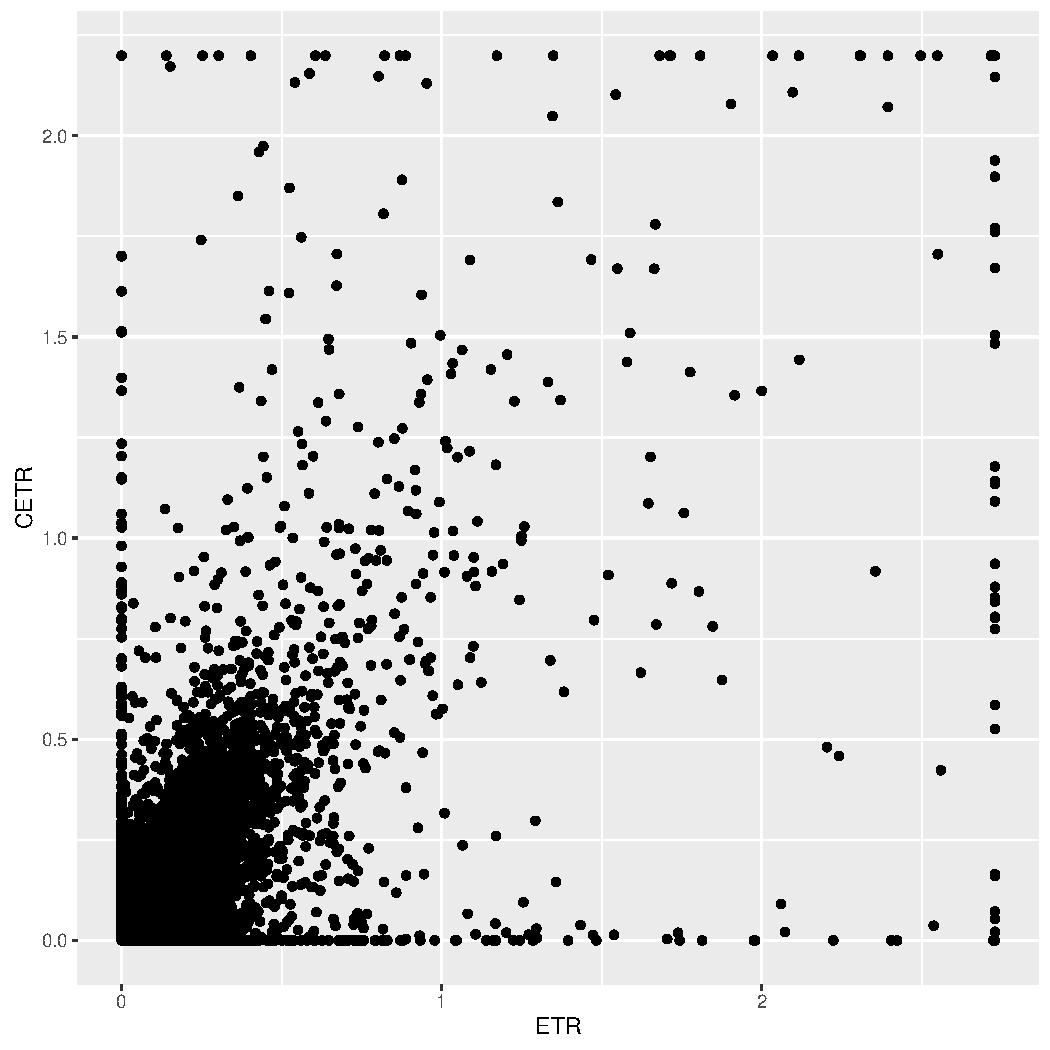
\includegraphics[width=\maxwidth]{figure/unnamed-chunk-1-1} 

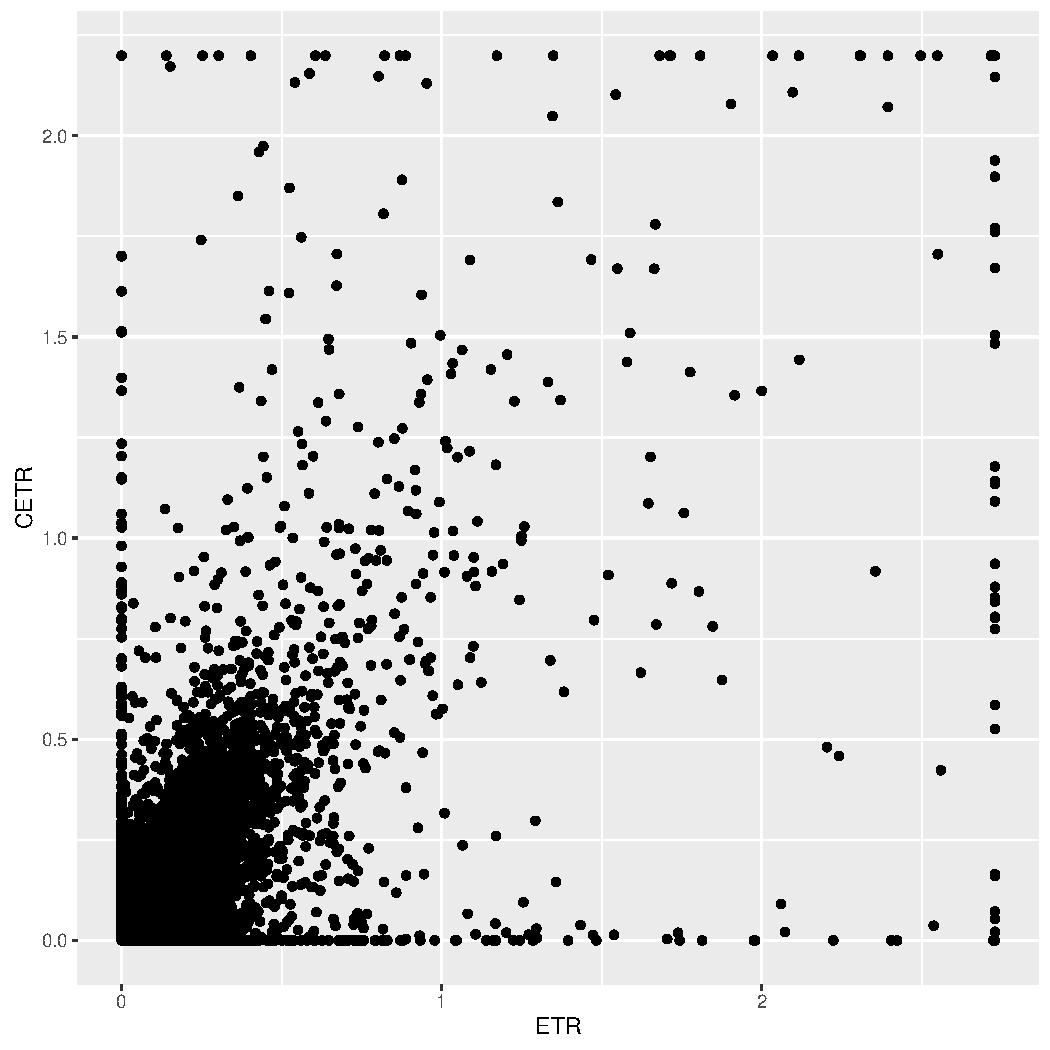
\includegraphics[width=\maxwidth]{figure/unnamed-chunk-1-2} 


\newpage
\section{\\Appendix D.2: Table of Market Structure(HHI)} \label{App:Appendix D.2}
\begin{knitrout}
\definecolor{shadecolor}{rgb}{0.969, 0.969, 0.969}\color{fgcolor}\begin{kframe}
\begin{alltt}
\hlstd{plottbA5} \hlkwb{<-} \hlkwa{function}\hlstd{(}\hlkwc{x}\hlstd{=TEJ8.1)\{}
  \hlstd{x}\hlopt{$}\hlstd{TSE} \hlkwb{<-} \hlkwd{paste}\hlstd{(x}\hlopt{$}\hlstd{TSE_code,x}\hlopt{$}\hlstd{TSE_name,}\hlkwc{sep}\hlstd{=}\hlstr{""}\hlstd{)}
  \hlstd{HHI_DB} \hlkwb{<-} \hlstd{base}\hlopt{::}\hlkwd{subset}\hlstd{(x,} \hlkwc{select}\hlstd{=}\hlkwd{c}\hlstd{(TSE,year,HHI))} \hlopt \hlstd{distinct}
  \hlstd{HHI_DB}\hlopt{$}\hlstd{HHI} \hlkwb{<-} \hlkwd{replace}\hlstd{(HHI_DB}\hlopt{$}\hlstd{HHI,HHI_DB}\hlopt{$}\hlstd{HHI} \hlopt{>=} \hlnum{0.3}\hlstd{,}\hlstr{'高寡佔I 型'}\hlstd{)}
  \hlstd{HHI_DB}\hlopt{$}\hlstd{HHI} \hlkwb{<-} \hlkwd{replace}\hlstd{(HHI_DB}\hlopt{$}\hlstd{HHI,HHI_DB}\hlopt{$}\hlstd{HHI} \hlopt{<} \hlnum{0.3} \hlopt{&} \hlstd{HHI_DB}\hlopt{$}\hlstd{HHI} \hlopt{>=} \hlnum{0.18}\hlstd{,}\hlstr{'高寡佔II 型'}\hlstd{)}
  \hlstd{HHI_DB}\hlopt{$}\hlstd{HHI} \hlkwb{<-} \hlkwd{replace}\hlstd{(HHI_DB}\hlopt{$}\hlstd{HHI,HHI_DB}\hlopt{$}\hlstd{HHI} \hlopt{<} \hlnum{0.18} \hlopt{&} \hlstd{HHI_DB}\hlopt{$}\hlstd{HHI} \hlopt{>=} \hlnum{0.14}\hlstd{,}\hlstr{'低寡占I 型'}\hlstd{)}
  \hlstd{HHI_DB}\hlopt{$}\hlstd{HHI} \hlkwb{<-} \hlkwd{replace}\hlstd{(HHI_DB}\hlopt{$}\hlstd{HHI,HHI_DB}\hlopt{$}\hlstd{HHI} \hlopt{<} \hlnum{0.14} \hlopt{&} \hlstd{HHI_DB}\hlopt{$}\hlstd{HHI} \hlopt{>=} \hlnum{0.1}\hlstd{,}\hlstr{'低寡占II 型'}\hlstd{)}
  \hlstd{HHI_DB}\hlopt{$}\hlstd{HHI} \hlkwb{<-} \hlkwd{replace}\hlstd{(HHI_DB}\hlopt{$}\hlstd{HHI,HHI_DB}\hlopt{$}\hlstd{HHI} \hlopt{<} \hlnum{0.1} \hlopt{&} \hlstd{HHI_DB}\hlopt{$}\hlstd{HHI} \hlopt{>=} \hlnum{0.05}\hlstd{,}\hlstr{'競爭I 型'}\hlstd{)}
  \hlstd{HHI_DB}\hlopt{$}\hlstd{HHI} \hlkwb{<-} \hlkwd{replace}\hlstd{(HHI_DB}\hlopt{$}\hlstd{HHI,HHI_DB}\hlopt{$}\hlstd{HHI} \hlopt{<} \hlnum{0.05}\hlstd{,}\hlstr{'競爭II 型'}\hlstd{)}
  \hlstd{HHI_DB}\hlopt{$}\hlstd{HHI} \hlkwb{<-} \hlkwd{replace}\hlstd{(HHI_DB}\hlopt{$}\hlstd{HHI,HHI_DB}\hlopt{$}\hlstd{HHI} \hlopt{==} \hlstr{"NaN"}\hlstd{,}\hlstr{""}\hlstd{)}
  \hlstd{HHI_tbl} \hlkwb{<-} \hlkwd{dcast}\hlstd{(HHI_DB,TSE} \hlopt{~} \hlstd{year)} \hlopt \hlstd{as.data.frame}
  \hlstd{HHI_tbl} \hlkwb{<-} \hlkwd{as.data.frame}\hlstd{(HHI_tbl[,}\hlopt{-}\hlnum{1}\hlstd{],}\hlkwc{row.names}\hlstd{=HHI_tbl[,}\hlnum{1}\hlstd{])}
  \hlkwd{return}\hlstd{(HHI_tbl)}
  \hlstd{\};HHI_tbl} \hlkwb{<-} \hlkwd{plottbA5}\hlstd{()}
\end{alltt}


{\ttfamily\noindent\itshape\color{messagecolor}{\#\# Using 'HHI' as value column. Use 'value.var' to override}}\end{kframe}
\end{knitrout}

\newpage
\newgeometry{margin=1cm}
\begin{landscape}
\thispagestyle{empty}

\begin{kframe}
\begin{alltt}
\hlkwd{print}\hlstd{(}\hlkwd{xtable}\hlstd{(HHI_tbl),}\hlkwc{scalebox}\hlstd{=}\hlnum{0.70}\hlstd{)}
\end{alltt}
\end{kframe}% latex table generated in R 3.3.1 by xtable 1.8-2 package
% Sat Oct 15 21:14:20 2016
\begin{table}[ht]
\centering
\scalebox{0.7}{
\begin{tabular}{rlllllllllllllll}
  \hline
 & 2001 & 2002 & 2003 & 2004 & 2005 & 2006 & 2007 & 2008 & 2009 & 2010 & 2011 & 2012 & 2013 & 2014 & 2015 \\ 
  \hline
M1100水泥工業 &  &  &  & 高寡佔I 型 & 高寡佔I 型 & 高寡佔I 型 & 高寡佔I 型 & 高寡佔I 型 & 高寡佔I 型 & 高寡佔I 型 & 高寡佔I 型 & 高寡佔I 型 & 高寡佔I 型 & 高寡佔I 型 & 高寡佔I 型 \\ 
  M1200食品工業 & 高寡佔II 型 & 高寡佔II 型 & 高寡佔II 型 & 高寡佔II 型 & 高寡佔II 型 & 高寡佔II 型 & 高寡佔II 型 & 高寡佔I 型 & 高寡佔I 型 & 高寡佔I 型 & 高寡佔I 型 & 高寡佔I 型 & 高寡佔I 型 & 高寡佔I 型 & 高寡佔I 型 \\ 
  M1300塑膠工業 &  & 高寡佔I 型 & 高寡佔I 型 & 高寡佔I 型 & 高寡佔I 型 & 高寡佔I 型 & 高寡佔II 型 & 高寡佔II 型 & 高寡佔II 型 & 高寡佔II 型 & 高寡佔II 型 & 高寡佔II 型 & 高寡佔II 型 & 高寡佔II 型 & 高寡佔II 型 \\ 
  M1400紡織纖維 & 競爭I 型 & 競爭I 型 & 競爭I 型 & 競爭I 型 & 競爭I 型 & 低寡占II 型 & 低寡占II 型 & 低寡占I 型 & 低寡占I 型 & 低寡占I 型 & 低寡占I 型 & 低寡占I 型 & 高寡佔II 型 & 高寡佔II 型 & 高寡佔II 型 \\ 
  M1500電機機械 & 高寡佔II 型 & 低寡占I 型 & 低寡占I 型 & 高寡佔II 型 & 低寡占I 型 & 高寡佔II 型 & 高寡佔II 型 & 高寡佔II 型 & 高寡佔II 型 & 高寡佔II 型 & 低寡占I 型 & 低寡占I 型 & 低寡占II 型 & 低寡占II 型 & 競爭I 型 \\ 
  M1600電器電纜 & 高寡佔II 型 & 高寡佔II 型 & 高寡佔II 型 & 高寡佔II 型 & 高寡佔II 型 & 高寡佔II 型 & 高寡佔II 型 & 高寡佔II 型 & 高寡佔II 型 & 高寡佔II 型 & 高寡佔I 型 & 高寡佔I 型 & 高寡佔I 型 & 高寡佔I 型 & 高寡佔I 型 \\ 
  M1721化學工業 & 高寡佔II 型 & 高寡佔II 型 & 低寡占I 型 & 低寡占I 型 & 低寡占II 型 & 低寡占II 型 & 競爭I 型 & 競爭I 型 & 競爭I 型 & 競爭I 型 & 競爭I 型 & 競爭I 型 & 競爭I 型 & 競爭I 型 & 競爭I 型 \\ 
  M1722生技醫療 &  & 高寡佔II 型 & 高寡佔II 型 & 低寡占I 型 & 低寡占II 型 & 低寡占II 型 & 競爭I 型 & 競爭I 型 & 競爭I 型 & 競爭I 型 & 競爭I 型 & 競爭I 型 & 競爭II 型 & 競爭II 型 & 競爭II 型 \\ 
  M1800玻璃陶瓷 &  &  &  &  &  &  &  &  &  &  &  & 高寡佔I 型 & 高寡佔I 型 & 高寡佔I 型 & 高寡佔I 型 \\ 
  M1900造紙工業 &  &  & 高寡佔I 型 & 高寡佔I 型 & 高寡佔I 型 & 高寡佔I 型 & 高寡佔I 型 & 高寡佔II 型 & 高寡佔II 型 & 高寡佔II 型 & 高寡佔II 型 & 高寡佔II 型 & 高寡佔II 型 & 高寡佔II 型 & 高寡佔II 型 \\ 
  M2000鋼鐵工業 & 高寡佔I 型 & 高寡佔II 型 & 高寡佔II 型 & 高寡佔II 型 & 高寡佔II 型 & 低寡占I 型 & 高寡佔II 型 & 高寡佔II 型 & 高寡佔II 型 & 高寡佔II 型 & 高寡佔II 型 & 高寡佔II 型 & 高寡佔II 型 & 高寡佔II 型 & 高寡佔II 型 \\ 
  M2100橡膠工業 &  &  &  & 高寡佔I 型 & 高寡佔II 型 & 高寡佔II 型 & 高寡佔II 型 & 高寡佔II 型 & 高寡佔II 型 & 高寡佔II 型 & 高寡佔II 型 & 高寡佔II 型 & 高寡佔II 型 & 高寡佔II 型 & 高寡佔II 型 \\ 
  M2200汽車工業 &  &  &  &  & 高寡佔II 型 & 高寡佔II 型 & 高寡佔II 型 & 高寡佔II 型 & 高寡佔II 型 & 高寡佔II 型 & 高寡佔II 型 & 高寡佔II 型 & 高寡佔II 型 & 高寡佔II 型 & 高寡佔II 型 \\ 
  M2324半導體 & 高寡佔I 型 & 高寡佔II 型 & 高寡佔II 型 & 高寡佔II 型 & 高寡佔II 型 & 低寡占II 型 & 競爭I 型 & 競爭I 型 & 競爭I 型 & 競爭I 型 & 競爭I 型 & 競爭I 型 & 競爭I 型 & 競爭I 型 & 低寡占II 型 \\ 
  M2325電腦及週邊 &  &  & 低寡占I 型 & 低寡占I 型 & 低寡占II 型 & 低寡占II 型 & 低寡占II 型 & 競爭I 型 & 競爭I 型 & 低寡占II 型 & 低寡占II 型 & 低寡占II 型 & 低寡占II 型 & 低寡占II 型 & 低寡占II 型 \\ 
  M2326光電業 & 高寡佔I 型 & 高寡佔I 型 & 高寡佔I 型 & 高寡佔II 型 & 高寡佔II 型 & 高寡佔II 型 & 低寡占II 型 & 低寡占II 型 & 低寡占II 型 & 低寡占II 型 & 低寡占II 型 & 低寡占II 型 & 低寡占II 型 & 低寡占II 型 & 低寡占II 型 \\ 
  M2327通信網路業 & 高寡佔I 型 & 高寡佔I 型 & 高寡佔I 型 & 高寡佔I 型 & 高寡佔I 型 & 高寡佔I 型 & 高寡佔II 型 & 低寡占II 型 & 低寡占II 型 & 低寡占II 型 & 低寡占II 型 & 低寡占II 型 & 低寡占II 型 & 低寡占II 型 & 低寡占II 型 \\ 
  M2328電子零組件 & 低寡占I 型 & 低寡占I 型 & 低寡占II 型 & 競爭I 型 & 競爭I 型 & 競爭II 型 & 競爭II 型 & 競爭II 型 & 競爭II 型 & 競爭II 型 & 競爭II 型 & 競爭II 型 & 競爭II 型 & 競爭II 型 & 競爭II 型 \\ 
  M2329電子通路業 &  &  & 低寡占II 型 & 競爭I 型 & 低寡占II 型 & 低寡占II 型 & 競爭I 型 & 競爭I 型 & 低寡占II 型 & 低寡占II 型 & 低寡占II 型 & 低寡占II 型 & 低寡占I 型 & 低寡占I 型 & 低寡占I 型 \\ 
  M2330資訊服務業 & 高寡佔II 型 & 高寡佔II 型 & 高寡佔II 型 & 高寡佔II 型 & 低寡占I 型 & 低寡占II 型 & 競爭I 型 & 競爭I 型 & 競爭I 型 & 競爭I 型 & 競爭I 型 & 競爭I 型 & 競爭I 型 & 競爭I 型 & 競爭I 型 \\ 
  M2500建材營造 & 低寡占II 型 & 低寡占II 型 & 競爭I 型 & 競爭I 型 & 競爭I 型 & 競爭I 型 & 競爭II 型 & 競爭II 型 & 競爭II 型 & 競爭II 型 & 競爭II 型 & 競爭II 型 & 競爭II 型 & 競爭II 型 & 競爭II 型 \\ 
  M2600航運業 &  & 高寡佔I 型 & 高寡佔I 型 & 高寡佔I 型 & 高寡佔I 型 & 高寡佔II 型 & 高寡佔II 型 & 低寡占I 型 & 低寡占I 型 & 低寡占I 型 & 低寡占I 型 & 低寡占I 型 & 低寡占I 型 & 低寡占I 型 & 低寡占I 型 \\ 
  M2700觀光事業 &  & 高寡佔II 型 & 高寡佔II 型 & 高寡佔II 型 & 低寡占I 型 & 低寡占I 型 & 低寡占II 型 & 低寡占II 型 & 低寡占II 型 & 低寡占II 型 & 低寡占II 型 & 低寡占II 型 & 低寡占II 型 & 低寡占II 型 & 低寡占II 型 \\ 
  M2900貿易百貨 &  & 高寡佔I 型 & 高寡佔I 型 & 高寡佔I 型 & 高寡佔I 型 & 高寡佔II 型 & 高寡佔II 型 & 高寡佔II 型 & 高寡佔II 型 & 高寡佔II 型 & 高寡佔II 型 & 高寡佔II 型 & 高寡佔II 型 & 高寡佔II 型 & 高寡佔II 型 \\ 
  M3200文化創意業 &  &  &  & 高寡佔II 型 & 高寡佔II 型 & 高寡佔II 型 & 高寡佔II 型 & 高寡佔II 型 & 高寡佔II 型 & 高寡佔II 型 & 高寡佔II 型 & 高寡佔II 型 & 高寡佔II 型 & 高寡佔II 型 & 高寡佔II 型 \\ 
  M9700油電燃氣業 & 高寡佔II 型 & 高寡佔II 型 & 高寡佔II 型 & 高寡佔I 型 & 高寡佔I 型 & 高寡佔I 型 & 高寡佔I 型 & 高寡佔I 型 & 高寡佔I 型 & 高寡佔I 型 & 高寡佔I 型 & 高寡佔I 型 & 高寡佔I 型 & 高寡佔I 型 & 高寡佔I 型 \\ 
   \hline
\end{tabular}
}
\end{table}


註:\\
a.分類方式參考美國司法部之市場結構分類標準,依HHI 值判斷其競爭程度,HHI 值愈小代表該產業集中度愈低,產業競爭程度愈激烈。\\
b.分類區間:高寡佔I 型≧0.3>高寡佔II 型≧0.18>低寡占I 型≧0.14>低寡占II 型≧0.1>競爭I 型≧0.05>競爭II 型。\\
\end{landscape}
\restoregeometry



\newpage
\newgeometry{margin=1cm}
\begin{landscape}
\thispagestyle{empty}
\section{\\Appendix D.3: Pearson Correlation Coefficiency} \label{App:Appendix D.3}
\begin{knitrout}
\definecolor{shadecolor}{rgb}{0.969, 0.969, 0.969}\color{fgcolor}\begin{kframe}
\begin{alltt}
\hlstd{ETR.cortab} \hlkwb{<-} \hlkwd{corstars}\hlstd{(TEJ8.1} \hlopt \hlkwd{select}\hlstd{(ETR,STR,HHI_Dum,ROA,SIZE,LEV,}
                     \hlstd{INTANG,QUICK,EQINC,OUTINSTI,RELAT,FAM_Dum,GDP)}
  \hlstd{,}\hlkwc{method} \hlstd{=} \hlstr{"pearson"}\hlstd{,}\hlkwc{removeTriangle} \hlstd{=} \hlstr{"lower"}\hlstd{,}\hlkwc{star} \hlstd{=} \hlnum{3}\hlstd{,}\hlkwc{result} \hlstd{=} \hlstr{"none"}\hlstd{)}
\end{alltt}


{\ttfamily\noindent\itshape\color{messagecolor}{\#\# Loading required package: Hmisc}}

{\ttfamily\noindent\itshape\color{messagecolor}{\#\# Loading required package: lattice}}

{\ttfamily\noindent\itshape\color{messagecolor}{\#\# Loading required package: survival}}

{\ttfamily\noindent\itshape\color{messagecolor}{\#\# Loading required package: Formula}}

{\ttfamily\noindent\itshape\color{messagecolor}{\#\# \\\#\# Attaching package: 'Hmisc'}}

{\ttfamily\noindent\itshape\color{messagecolor}{\#\# The following objects are masked from 'package:dplyr':\\\#\# \\\#\#\ \ \ \  combine, src, summarize}}

{\ttfamily\noindent\itshape\color{messagecolor}{\#\# The following objects are masked from 'package:xtable':\\\#\# \\\#\#\ \ \ \  label, label<-}}

{\ttfamily\noindent\itshape\color{messagecolor}{\#\# The following objects are masked from 'package:base':\\\#\# \\\#\#\ \ \ \  format.pval, round.POSIXt, trunc.POSIXt, units}}\begin{alltt}
\hlstd{CETR.cortab} \hlkwb{<-} \hlkwd{corstars}\hlstd{(TEJ8.1} \hlopt \hlkwd{select}\hlstd{(CETR,STR,HHI_Dum,ROA,SIZE,LEV,}
                     \hlstd{INTANG,QUICK,EQINC,OUTINSTI,RELAT,FAM_Dum,GDP)}
  \hlstd{,}\hlkwc{method} \hlstd{=} \hlstr{"pearson"}\hlstd{,}\hlkwc{removeTriangle} \hlstd{=} \hlstr{"lower"}\hlstd{,}\hlkwc{star} \hlstd{=} \hlnum{3}\hlstd{,}\hlkwc{result} \hlstd{=} \hlstr{"none"}\hlstd{)}
\end{alltt}
\end{kframe}
\end{knitrout}
\end{landscape}


\newpage
\begin{landscape}
\thispagestyle{empty}
\centerline{表、相關係數表(應變數為ETR)}
\begin{kframe}
\begin{alltt}
 \hlkwd{xtable}\hlstd{(ETR.cortab)}
\end{alltt}
\end{kframe}% latex table generated in R 3.3.1 by xtable 1.8-2 package
% Sat Oct 15 21:14:24 2016
\begin{table}[ht]
\centering
\begin{tabular}{rlllllllllllll}
  \hline
 & ETR & STR & HHI\_Dum & ROA & SIZE & LEV & INTANG & QUICK & EQINC & OUTINSTI & RELAT & FAM\_Dum & GDP \\ 
  \hline
ETR &  1.00  &  0.01    & -0.03**  &  0.06*** &  0.02**  &  0.02*   &  0.01    & -0.02*   & -0.01    & -0.05*** &  0.00    &  0.01    &  0.04*** \\ 
  STR &  &  1.00  &  0.05*** & -0.03*** & -0.11*** & -0.11*** &  0.05*** &  0.09*** &  0.00    & -0.11*** &  0.01    & -0.02**  &  0.22*** \\ 
  HHI\_Dum &  &  &  1.00  & -0.01    & -0.09*** & -0.07*** &  0.01    &  0.08*** & -0.04*** & -0.05*** &  0.04*** &  0.00    &  0.16*** \\ 
  ROA &  &  &  &  1.00  &  0.10*** & -0.26*** & -0.04*** &  0.09*** &  0.17*** &  0.17*** &  0.01    & -0.05*** & -0.03*** \\ 
  SIZE &  &  &  &  &  1.00  &  0.29*** &  0.04*** & -0.21*** &  0.16*** &  0.39*** &  0.02**  &  0.03*** &  0.08*** \\ 
  LEV &  &  &  &  &  &  1.00  & -0.06*** & -0.57*** & -0.04*** &  0.04*** &  0.03*** &  0.06*** & -0.08*** \\ 
  INTANG &  &  &  &  &  &  &  1.00  &  0.05*** & -0.03*** &  0.05*** &  0.00    &  0.01    &  0.06*** \\ 
  QUICK &  &  &  &  &  &  &  &  1.00  &  0.01    & -0.02*   & -0.01    & -0.08*** &  0.08*** \\ 
  EQINC &  &  &  &  &  &  &  &  &  1.00  &  0.12*** &  0.00    &  0.00    &  0.08*** \\ 
  OUTINSTI &  &  &  &  &  &  &  &  &  &  1.00  & -0.01    & -0.04*** &  0.07*** \\ 
  RELAT &  &  &  &  &  &  &  &  &  &  &  1.00  & -0.02*   & -0.03*** \\ 
  FAM\_Dum &  &  &  &  &  &  &  &  &  &  &  &  1.00  & -0.01    \\ 
  GDP &  &  &  &  &  &  &  &  &  &  &  &  &  1.00  \\ 
   \hline
\end{tabular}
\end{table}

註:a. 變數定義同前表。\\
    b. ***、**、*表示1\%、5\% 及10\% 顯著水準。\\
\end{landscape}

\newpage
\begin{landscape}
\centerline{表、相關係數表(應變數為CETR)}
\begin{kframe}
\begin{alltt}
\hlkwd{xtable}\hlstd{(CETR.cortab)}
\end{alltt}
\end{kframe}% latex table generated in R 3.3.1 by xtable 1.8-2 package
% Sat Oct 15 21:14:24 2016
\begin{table}[ht]
\centering
\begin{tabular}{rlllllllllllll}
  \hline
 & CETR & STR & HHI\_Dum & ROA & SIZE & LEV & INTANG & QUICK & EQINC & OUTINSTI & RELAT & FAM\_Dum & GDP \\ 
  \hline
CETR &  1.00  &  0.02*   & -0.02**  &  0.02**  &  0.02*   &  0.02*   &  0.02    & -0.03*** & -0.02**  & -0.06*** &  0.00    &  0.02*   &  0.04*** \\ 
  STR &  &  1.00  &  0.05*** & -0.03*** & -0.11*** & -0.11*** &  0.05*** &  0.09*** &  0.00    & -0.11*** &  0.01    & -0.02**  &  0.22*** \\ 
  HHI\_Dum &  &  &  1.00  & -0.01    & -0.09*** & -0.07*** &  0.01    &  0.08*** & -0.04*** & -0.05*** &  0.04*** &  0.00    &  0.16*** \\ 
  ROA &  &  &  &  1.00  &  0.10*** & -0.26*** & -0.04*** &  0.09*** &  0.17*** &  0.17*** &  0.01    & -0.05*** & -0.03*** \\ 
  SIZE &  &  &  &  &  1.00  &  0.29*** &  0.04*** & -0.21*** &  0.16*** &  0.39*** &  0.02**  &  0.03*** &  0.08*** \\ 
  LEV &  &  &  &  &  &  1.00  & -0.06*** & -0.57*** & -0.04*** &  0.04*** &  0.03*** &  0.06*** & -0.08*** \\ 
  INTANG &  &  &  &  &  &  &  1.00  &  0.05*** & -0.03*** &  0.05*** &  0.00    &  0.01    &  0.06*** \\ 
  QUICK &  &  &  &  &  &  &  &  1.00  &  0.01    & -0.02*   & -0.01    & -0.08*** &  0.08*** \\ 
  EQINC &  &  &  &  &  &  &  &  &  1.00  &  0.12*** &  0.00    &  0.00    &  0.08*** \\ 
  OUTINSTI &  &  &  &  &  &  &  &  &  &  1.00  & -0.01    & -0.04*** &  0.07*** \\ 
  RELAT &  &  &  &  &  &  &  &  &  &  &  1.00  & -0.02*   & -0.03*** \\ 
  FAM\_Dum &  &  &  &  &  &  &  &  &  &  &  &  1.00  & -0.01    \\ 
  GDP &  &  &  &  &  &  &  &  &  &  &  &  &  1.00  \\ 
   \hline
\end{tabular}
\end{table}

註:a. 變數定義同前表。\\
    b. ***、**、*表示1\%、5\% 及10\% 顯著水準。\\

\end{landscape}

\newpage
\begin{knitrout}
\definecolor{shadecolor}{rgb}{0.969, 0.969, 0.969}\color{fgcolor}\begin{kframe}
\begin{alltt}
\hlstd{lm.ETR} \hlkwb{<-} \hlkwd{lm}\hlstd{(ETR} \hlopt{~} \hlstd{STR}\hlopt{+}\hlstd{HHI_Dum}\hlopt{+}\hlstd{ROA}\hlopt{+}\hlstd{SIZE}\hlopt{+}\hlstd{LEV}\hlopt{+}\hlstd{INTANG}\hlopt{+}\hlstd{QUICK}\hlopt{+}\hlstd{EQINC}\hlopt{+}\hlstd{OUTINSTI}\hlopt{+}\hlstd{RELAT}\hlopt{+}\hlstd{FAM_Dum}\hlopt{+}\hlstd{GDP}
            \hlstd{,TEJ8.1)}
\hlstd{lm.CETR} \hlkwb{<-} \hlkwd{lm}\hlstd{(CETR} \hlopt{~} \hlstd{STR}\hlopt{+}\hlstd{HHI_Dum}\hlopt{+}\hlstd{ROA}\hlopt{+}\hlstd{SIZE}\hlopt{+}\hlstd{LEV}\hlopt{+}\hlstd{INTANG}\hlopt{+}\hlstd{QUICK}\hlopt{+}\hlstd{EQINC}\hlopt{+}\hlstd{OUTINSTI}\hlopt{+}\hlstd{RELAT}\hlopt{+}\hlstd{FAM_Dum}\hlopt{+}\hlstd{GDP}
             \hlstd{,TEJ8.1)}
\hlstd{lm.ETR.SH} \hlkwb{<-} \hlkwd{lm}\hlstd{(ETR} \hlopt{~} \hlstd{STR}\hlopt{+}\hlstd{HHI_Dum}\hlopt{+}\hlstd{STR_HHI}\hlopt{+}\hlstd{ROA}\hlopt{+}\hlstd{SIZE}\hlopt{+}\hlstd{LEV}\hlopt{+}\hlstd{INTANG}\hlopt{+}\hlstd{QUICK}\hlopt{+}\hlstd{EQINC}\hlopt{+}\hlstd{OUTINSTI}\hlopt{+}\hlstd{RELAT}\hlopt{+}\hlstd{FAM_Dum}\hlopt{+}\hlstd{GDP,TEJ8.1)}
\hlstd{lm.CETR.SH} \hlkwb{<-} \hlkwd{lm}\hlstd{(CETR} \hlopt{~} \hlstd{STR}\hlopt{+}\hlstd{HHI_Dum}\hlopt{+}\hlstd{STR_HHI}\hlopt{+}\hlstd{ROA}\hlopt{+}\hlstd{SIZE}\hlopt{+}\hlstd{LEV}\hlopt{+}\hlstd{INTANG}\hlopt{+}\hlstd{QUICK}\hlopt{+}\hlstd{EQINC}\hlopt{+}\hlstd{OUTINSTI}\hlopt{+}\hlstd{RELAT}\hlopt{+}\hlstd{FAM_Dum}\hlopt{+}\hlstd{GDP,TEJ8.1)}
\end{alltt}
\end{kframe}
\end{knitrout}

\newpage
\section{\\Appendix F.1: Empirical - 1} \label{App:Appendix F.1}
模型1:\\
$TAXAVO_{it}=\beta_{0}+\beta_{1}STR_{it}+\beta_{2}HHI_{jt}+\beta_{3}ROA_{it}+\beta_{4}SIZE_{it}+\beta_{5}LEV_{it}+\beta_{6}INTANG_{it}+\beta_{7}QUICK_{it}+\beta_{8}EQINC_{it}+\beta_{9}OUTINSTI_{it}+\beta_{10}RELAT_{it}+\beta_{11}FAMILY_{it}+\beta_{12}GDP_{it}+\varepsilon_{13}$\\
實證結果─不包含STRATEGY×HHI\\
\begin{kframe}
\begin{alltt}
  \hlkwd{stargazer}\hlstd{(lm.ETR,lm.CETR,}
    \hlkwc{dep.var.labels} \hlstd{=} \hlkwd{c}\hlstd{(}\hlstr{"$TAXAVO_\{it\}=ETR_\{it\}$"}\hlstd{,}\hlstr{"$TAXAVO_\{it\}=CashETR_\{it\}$"}\hlstd{),}
    \hlkwc{digits}\hlstd{=}\hlnum{3}\hlstd{)}
\end{alltt}
\end{kframe}
% Table created by stargazer v.5.2 by Marek Hlavac, Harvard University. E-mail: hlavac at fas.harvard.edu
% Date and time: 週六, 十月 15, 2016 - 下午 09:14:25
\begin{table}[!htbp] \centering 
  \caption{} 
  \label{} 
\begin{tabular}{@{\extracolsep{5pt}}lcc} 
\\[-1.8ex]\hline 
\hline \\[-1.8ex] 
 & \multicolumn{2}{c}{\textit{Dependent variable:}} \\ 
\cline{2-3} 
\\[-1.8ex] & $TAXAVO_{it}=ETR_{it}$ & $TAXAVO_{it}=CashETR_{it}$ \\ 
\\[-1.8ex] & (1) & (2)\\ 
\hline \\[-1.8ex] 
 STR & $-$0.0002 & 0.0003 \\ 
  & (0.0004) & (0.0004) \\ 
  & & \\ 
 HHI\_Dum & $-$0.018$^{***}$ & $-$0.014$^{***}$ \\ 
  & (0.004) & (0.004) \\ 
  & & \\ 
 ROA & 0.210$^{***}$ & 0.107$^{***}$ \\ 
  & (0.022) & (0.020) \\ 
  & & \\ 
 SIZE & 0.006$^{***}$ & 0.005$^{***}$ \\ 
  & (0.002) & (0.002) \\ 
  & & \\ 
 LEV & 0.043$^{***}$ & 0.019 \\ 
  & (0.015) & (0.014) \\ 
  & & \\ 
 INTANG & 0.121$^{*}$ & 0.144$^{**}$ \\ 
  & (0.070) & (0.063) \\ 
  & & \\ 
 QUICK & $-$0.001 & $-$0.002$^{**}$ \\ 
  & (0.001) & (0.001) \\ 
  & & \\ 
 EQINC & $-$0.782$^{***}$ & $-$0.942$^{***}$ \\ 
  & (0.289) & (0.260) \\ 
  & & \\ 
 OUTINSTI & $-$0.095$^{***}$ & $-$0.083$^{***}$ \\ 
  & (0.010) & (0.009) \\ 
  & & \\ 
 RELAT & $-$0.0001 & 0.0001 \\ 
  & (0.0002) & (0.0002) \\ 
  & & \\ 
 FAM\_Dum & 0.006 & 0.006$^{*}$ \\ 
  & (0.004) & (0.004) \\ 
  & & \\ 
 GDP & 0.100$^{***}$ & 0.080$^{***}$ \\ 
  & (0.015) & (0.013) \\ 
  & & \\ 
 Constant & $-$1.539$^{***}$ & $-$1.223$^{***}$ \\ 
  & (0.240) & (0.216) \\ 
  & & \\ 
\hline \\[-1.8ex] 
Observations & 15,483 & 15,483 \\ 
R$^{2}$ & 0.014 & 0.011 \\ 
Adjusted R$^{2}$ & 0.013 & 0.011 \\ 
Residual Std. Error (df = 15470) & 0.259 & 0.233 \\ 
F Statistic (df = 12; 15470) & 18.272$^{***}$ & 14.713$^{***}$ \\ 
\hline 
\hline \\[-1.8ex] 
\textit{Note:}  & \multicolumn{2}{r}{$^{*}$p$<$0.1; $^{**}$p$<$0.05; $^{***}$p$<$0.01} \\ 
\end{tabular} 
\end{table} 


\newpage
\section{\\Appendix F.2: Empirical - 2} \label{App:Appendix F.2}
模型2:\\
$TAXAVO_{it}=\beta_{0}+\beta_{1}STR_{it}+\beta_{2}HHI_{jt}+\beta_{3}ROA_{it}+\beta_{4}SIZE_{it}+\beta_{5}LEV_{it}+\beta_{6}INTANG_{it}+\beta_{7}QUICK_{it}+\beta_{8}EQINC_{it}+\beta_{9}OUTINSTI_{it}+\beta_{10}RELAT_{it}+\beta_{11}FAMILY_{it}+\beta_{12}GDP_{it}+\varepsilon_{13}$\\
實證結果─包含STRATEGY×HHI\\
\begin{kframe}
\begin{alltt}
  \hlkwd{stargazer}\hlstd{(lm.ETR.SH,lm.CETR.SH,}
    \hlkwc{dep.var.labels} \hlstd{=} \hlkwd{c}\hlstd{(}\hlstr{"TAXAVO_\{it\}=ETR_\{it\}"}\hlstd{,}\hlstr{"TAXAVO_\{it\}=CashETR_\{it\}"}\hlstd{),}
    \hlkwc{digits}\hlstd{=}\hlnum{3}\hlstd{)}
\end{alltt}
\end{kframe}
% Table created by stargazer v.5.2 by Marek Hlavac, Harvard University. E-mail: hlavac at fas.harvard.edu
% Date and time: 週六, 十月 15, 2016 - 下午 09:14:26
\begin{table}[!htbp] \centering 
  \caption{} 
  \label{} 
\begin{tabular}{@{\extracolsep{5pt}}lcc} 
\\[-1.8ex]\hline 
\hline \\[-1.8ex] 
 & \multicolumn{2}{c}{\textit{Dependent variable:}} \\ 
\cline{2-3} 
\\[-1.8ex] & TAXAVO_{it}=ETR_{it} & TAXAVO_{it}=CashETR_{it} \\ 
\\[-1.8ex] & (1) & (2)\\ 
\hline \\[-1.8ex] 
 STR & 0.0002 & 0.001$^{*}$ \\ 
  & (0.001) & (0.0005) \\ 
  & & \\ 
 HHI\_Dum & 0.0001 & 0.006 \\ 
  & (0.013) & (0.012) \\ 
  & & \\ 
 STR\_HHI & $-$0.001 & $-$0.001$^{*}$ \\ 
  & (0.001) & (0.001) \\ 
  & & \\ 
 ROA & 0.210$^{***}$ & 0.107$^{***}$ \\ 
  & (0.022) & (0.020) \\ 
  & & \\ 
 SIZE & 0.006$^{***}$ & 0.005$^{***}$ \\ 
  & (0.002) & (0.002) \\ 
  & & \\ 
 LEV & 0.043$^{***}$ & 0.018 \\ 
  & (0.015) & (0.014) \\ 
  & & \\ 
 INTANG & 0.127$^{*}$ & 0.150$^{**}$ \\ 
  & (0.070) & (0.063) \\ 
  & & \\ 
 QUICK & $-$0.001 & $-$0.002$^{**}$ \\ 
  & (0.001) & (0.001) \\ 
  & & \\ 
 EQINC & $-$0.791$^{***}$ & $-$0.952$^{***}$ \\ 
  & (0.289) & (0.260) \\ 
  & & \\ 
 OUTINSTI & $-$0.095$^{***}$ & $-$0.083$^{***}$ \\ 
  & (0.010) & (0.009) \\ 
  & & \\ 
 RELAT & $-$0.00005 & 0.0001 \\ 
  & (0.0002) & (0.0002) \\ 
  & & \\ 
 FAM\_Dum & 0.006 & 0.006$^{*}$ \\ 
  & (0.004) & (0.004) \\ 
  & & \\ 
 GDP & 0.098$^{***}$ & 0.078$^{***}$ \\ 
  & (0.015) & (0.013) \\ 
  & & \\ 
 Constant & $-$1.511$^{***}$ & $-$1.192$^{***}$ \\ 
  & (0.241) & (0.216) \\ 
  & & \\ 
\hline \\[-1.8ex] 
Observations & 15,483 & 15,483 \\ 
R$^{2}$ & 0.014 & 0.011 \\ 
Adjusted R$^{2}$ & 0.013 & 0.011 \\ 
Residual Std. Error (df = 15469) & 0.259 & 0.233 \\ 
F Statistic (df = 13; 15469) & 17.035$^{***}$ & 13.837$^{***}$ \\ 
\hline 
\hline \\[-1.8ex] 
\textit{Note:}  & \multicolumn{2}{r}{$^{*}$p$<$0.1; $^{**}$p$<$0.05; $^{***}$p$<$0.01} \\ 
\end{tabular} 
\end{table} 


\newpage
敏感性分析\\
分析一、百分位\\

\begin{kframe}
\begin{alltt}
  \hlstd{TEJ8.2} \hlkwb{<-} \hlstd{TEJ8.1} \hlopt \hlkwd{mutate}\hlstd{(}\hlkwc{STR.PR} \hlstd{= STR_RD.perank}\hlopt{+}\hlstd{STR_MB.perank}\hlopt{+}\hlstd{STR_EMP.perank}\hlopt{+}\hlstd{STR_PPE.perank}\hlopt{+}\hlstd{STR_MARKET.perank)} \hlopt \hlkwd{mutate}\hlstd{(}\hlkwc{STR.PR_HHI} \hlstd{= STR.PR}\hlopt{*}\hlstd{HHI_Dum)}

  \hlkwd{stargazer}\hlstd{(TEJ8.2} \hlopt \hlkwd{select}\hlstd{(ETR,STR.PR,HHI_Dum,STR.PR_HHI,ROA,SIZE,LEV,INTANG,QUICK,EQINC,OUTINSTI,RELAT,FAM_Dum,GDP),}
            \hlkwc{type} \hlstd{=} \hlstr{"latex"}\hlstd{)}
\end{alltt}
\end{kframe}
% Table created by stargazer v.5.2 by Marek Hlavac, Harvard University. E-mail: hlavac at fas.harvard.edu
% Date and time: 週六, 十月 15, 2016 - 下午 09:14:26
\begin{table}[!htbp] \centering 
  \caption{} 
  \label{} 
\begin{tabular}{@{\extracolsep{5pt}}lccccc} 
\\[-1.8ex]\hline 
\hline \\[-1.8ex] 
Statistic & \multicolumn{1}{c}{N} & \multicolumn{1}{c}{Mean} & \multicolumn{1}{c}{St. Dev.} & \multicolumn{1}{c}{Min} & \multicolumn{1}{c}{Max} \\ 
\hline \\[-1.8ex] 
ETR & 15,570 & 0.175 & 0.260 & 0.000 & 2.728 \\ 
STR.PR & 14,454 & 2.500 & 0.771 & 0.351 & 4.972 \\ 
HHI\_Dum & 15,483 & 0.388 & 0.487 & 0 & 1 \\ 
STR.PR\_HHI & 14,454 & 0.989 & 1.316 & 0.000 & 4.807 \\ 
ROA & 15,570 & 0.045 & 0.103 & $-$0.467 & 0.343 \\ 
SIZE & 15,570 & 15.199 & 1.421 & 12.310 & 19.948 \\ 
LEV & 15,570 & 0.416 & 0.178 & 0.041 & 0.904 \\ 
INTANG & 15,570 & 0.013 & 0.030 & 0.000 & 0.250 \\ 
QUICK & 15,570 & 1.884 & 2.415 & 0.036 & 21.571 \\ 
EQINC & 15,570 & 0.0002 & 0.007 & $-$0.040 & 0.050 \\ 
OUTINSTI & 15,570 & 0.365 & 0.227 & 0.000 & 1.000 \\ 
RELAT & 15,570 & 2.257 & 9.555 & 0.000 & 100.000 \\ 
FAM\_Dum & 15,570 & 0.611 & 0.488 & 0 & 1 \\ 
GDP & 15,570 & 16.382 & 0.149 & 16.019 & 16.564 \\ 
\hline \\[-1.8ex] 
\end{tabular} 
\end{table} 


\newpage
\begin{kframe}
\begin{alltt}
  \hlkwd{stargazer}\hlstd{(TEJ8.2} \hlopt \hlkwd{select}\hlstd{(CETR,STR.PR,HHI_Dum,STR.PR_HHI,ROA,SIZE,LEV,INTANG,QUICK,EQINC,OUTINSTI,RELAT,FAM_Dum,GDP),}
            \hlkwc{type} \hlstd{=} \hlstr{"latex"}\hlstd{)}
\end{alltt}
\end{kframe}
% Table created by stargazer v.5.2 by Marek Hlavac, Harvard University. E-mail: hlavac at fas.harvard.edu
% Date and time: 週六, 十月 15, 2016 - 下午 09:14:27
\begin{table}[!htbp] \centering 
  \caption{} 
  \label{} 
\begin{tabular}{@{\extracolsep{5pt}}lccccc} 
\\[-1.8ex]\hline 
\hline \\[-1.8ex] 
Statistic & \multicolumn{1}{c}{N} & \multicolumn{1}{c}{Mean} & \multicolumn{1}{c}{St. Dev.} & \multicolumn{1}{c}{Min} & \multicolumn{1}{c}{Max} \\ 
\hline \\[-1.8ex] 
CETR & 15,570 & 0.157 & 0.234 & 0.000 & 2.199 \\ 
STR.PR & 14,454 & 2.500 & 0.771 & 0.351 & 4.972 \\ 
HHI\_Dum & 15,483 & 0.388 & 0.487 & 0 & 1 \\ 
STR.PR\_HHI & 14,454 & 0.989 & 1.316 & 0.000 & 4.807 \\ 
ROA & 15,570 & 0.045 & 0.103 & $-$0.467 & 0.343 \\ 
SIZE & 15,570 & 15.199 & 1.421 & 12.310 & 19.948 \\ 
LEV & 15,570 & 0.416 & 0.178 & 0.041 & 0.904 \\ 
INTANG & 15,570 & 0.013 & 0.030 & 0.000 & 0.250 \\ 
QUICK & 15,570 & 1.884 & 2.415 & 0.036 & 21.571 \\ 
EQINC & 15,570 & 0.0002 & 0.007 & $-$0.040 & 0.050 \\ 
OUTINSTI & 15,570 & 0.365 & 0.227 & 0.000 & 1.000 \\ 
RELAT & 15,570 & 2.257 & 9.555 & 0.000 & 100.000 \\ 
FAM\_Dum & 15,570 & 0.611 & 0.488 & 0 & 1 \\ 
GDP & 15,570 & 16.382 & 0.149 & 16.019 & 16.564 \\ 
\hline \\[-1.8ex] 
\end{tabular} 
\end{table} 


%\end{CJK}
\end{document}
